\documentclass[11pt]{beamer}
\mode<presentation>
\let\Tiny=\tiny
\usetheme{CambridgeUS}
\usefonttheme{professionalfonts}
\usepackage[brazil]{babel}
\usepackage[utf8]{inputenc}
\newtheorem{mydef}{Definição}
\newtheorem{myexample}{Exemplo}

\title{Processo de \textit{Software}}
\author{}
\date{}

\begin{document}

   \begin{frame}[plain]
        \titlepage
   \end{frame}

   \section*{Introdução}

   \begin{frame}{Processo de \textit{software}}
      \begin{itemize}
         \item A Engenharia de \textit{Software}, na quase totalidade de sua existência, focou-se em traduzir sistemas de informação já existentes para o computador.
         \item Por isso, a literatura especializada dá maior relevância ao processo de desenvolvimento em si.
         \item Isto é justificado porque, se os processos de negócio já existem e são maduros, então o resultado final fica a cargo da implementação correta do processo.
      \end{itemize}
   \end{frame}

   \begin{frame}{Métodos orientados a planos $\times$ métodos ágeis}
      \begin{itemize}
         \item Nos últimos 20 anos, há um grande embate dentro da Engenharia de \textit{Software} entre métodos orientados a planos e os novos métodos ágeis.
         \item Os métodos orientados a planos são métodos dentro do processo de desenvolvimento de \textit{software} mais antigos e que se baseiam no máximo planejamento.
         \item Abordaremos aqui os processos de \textit{software} de acordo com este paradigma.
      \end{itemize}
   \end{frame}

   \begin{frame}{Atividades do processo de \textit{software}}
      Os diferentes modelos de processo de desenvolvimento de \textit{software} baseiam-se geralmente nas seguintes atividades:
      \begin{itemize}
         \item especificação;
         \item projeto e implementação;
         \item validação;
         \item evolução.
      \end{itemize}
      Cada uma destas atividades é composta por outras inúmeras atividades, como documentação e gerenciamento de configuração de \textit{software}.
   \end{frame}

   \section{Modelos de processo}

   \begin{frame}{Modelos de processo}
      Devido à complexidade do processo de \textit{software}, pode-se representá-lo através de modelos, representações simplificadas do processo. Alguns dos principais modelos são:
      \begin{itemize}
         \item cascata;
         \item desenvolvimento incremental.
      \end{itemize}
      Os modelos também são chamados de paradigmas de processo.
   \end{frame}

   \begin{frame}{Modelo cascata}
      \begin{itemize}
         \item O modelo cascata é o modelo clássico para o desenvolvimento de \textit{software}.
         \item Ele e o Rational Unified Process (RUP) são os modelos mais emblemáticos dos métodos orientados a planos.
      \end{itemize}
   \end{frame}

   \begin{frame}{Modelo cascata}
      \begin{itemize}
         \item É formado por atividades encadeadas, onde uma atividade só pode ser executada caso uma atividade anterior seja terminada.
         \item Exige um extenso planejamento prévio das atividades.
         \item É composto pelas seguintes atividades:
           \begin{itemize}
              \item análise e definição de requisitos;
              \item projeto de sistema e \textit{software};
              \item implementação e teste unitário
              \item teste de integração e de sistema;
              \item operação e manutenção.
           \end{itemize}
      \end{itemize}
   \end{frame}

   \begin{frame}{Modelo cascata}
      \begin{figure}[ht]
        \centering
        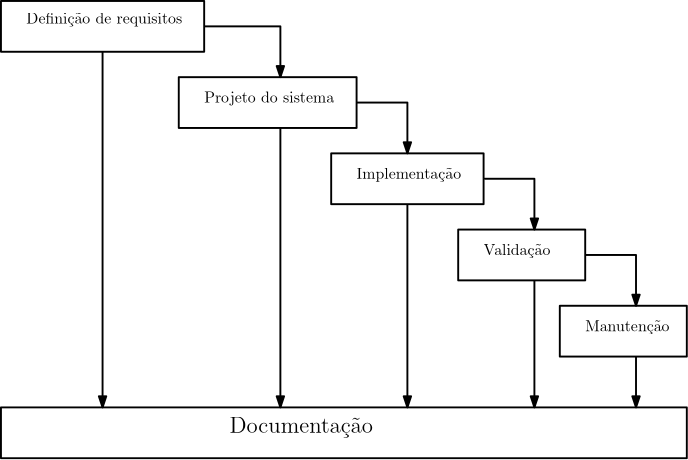
\includegraphics[height=6.6cm, width=9cm]{figures/cascata.png}
      \end{figure}
   \end{frame}

   \begin{frame}{Modelo cascata}
      \begin{itemize}
         \item Cada fase do modelo cascata gera documentos que validam a fase.
         \item Erros ou modificações nos requisitos fazem com que o processo retorne a etapas anteriores.
         \item As fases iniciais não produzem \textit{software}, apenas documentação.
         \item O cliente só recebe um produto funcional ao fim das etapas.
      \end{itemize}
   \end{frame}

   \begin{frame}{Modelo cascata}
      \begin{itemize}
         \item O modelo não reage bem a mudanças nos requisitos devido à sua natureza conservadora.
         \item Projetos reais nem sempre seguem o modelo à risca.
         \item Nem sempre todos os requisitos são conhecidos no início do projeto.
         \item Em um ambiente de negócios dinâmico tende a ser ineficiente.
      \end{itemize}
   \end{frame}

   \begin{frame}{Modelo cascata}
       \begin{itemize}
          \item Alguns contratos, como os firmados com governos, exigem ainda um processo em cascata.
          \item \textit{Softwares} embarcados e sistemas críticos o cascata encontra bastante espaço.
          \item \textit{Softwares} produzidos em trabalhos acadêmicos, onde a equipe de pesquisa é também a de desenvolvimento, o cascata também é utilizado, mesmo que de maneira menos formal.
       \end{itemize}
   \end{frame}

   \begin{frame}{Desenvolvimento incremental}
       \begin{itemize}
          \item O desenvolvimento incremental divide o processo de desenvolvimento de \textit{software} em iterações.
          \item Em cada iteração, a versão do \textit{software} é posta para validação com o cliente.
          \item As versões intermediárias não possuem todas as funcionalidades requeridas, apenas as necessárias para se obter um \textit{software} funcional.
          \item Este modelo serve tanto para abordagens orientadas a planos quanto para métodos ágeis.
       \end{itemize}
   \end{frame}

   \begin{frame}{Desenvolvimento incremental}
       Cada iteração é dividida nas seguintes etapas:
       \begin{itemize}
          \item especificação;
          \item desenvolvimento;
          \item validação.
       \end{itemize}
   \end{frame}

   \begin{frame}{Desenvolvimento incremental}
      \begin{figure}[ht]
        \centering
        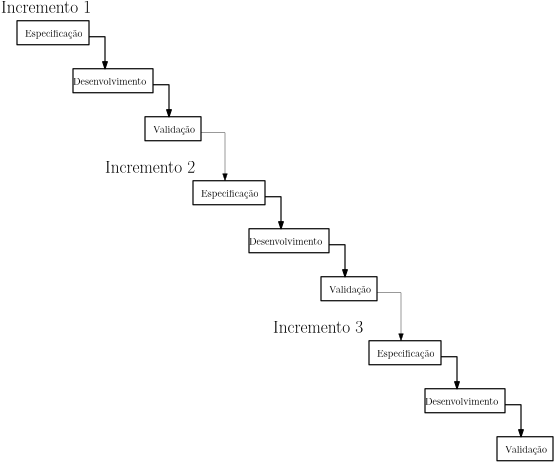
\includegraphics[height=6.7cm, width=11cm]{figures/incremental.png}
      \end{figure}
   \end{frame}

   \begin{frame}{Desenvolvimento incremental}
      \begin{itemize}
         \item Muito mais dinâmico e capacidade de tolerar erros e mudanças que o modelo cascata.
         \item Os custos das mudanças de requisitos são reduzidos.
         \item O \textit{feedback} constante do cliente ajuda a prevenir erros de identificação de requisitos.
         \item É o modelo adotado em larga escala pela Engenharia de \textit{Software} moderna, em especial na criação de produtos de \textit{software} (próxima aula) e nos métodos ágeis.
      \end{itemize}
   \end{frame}

   \begin{frame}{Desenvolvimento incremental}
      \begin{itemize}
         \item Há a necessidade de mensurar, de maneira correta, o tamanho das iterações.
         \item Iterações longas degeneram o processo em um modelo em cascata.
         \item Iterações curtas geram \textit{overhead} com mais validações e planejamentos, além de gerar prazos mais curtos à equipe.
      \end{itemize}
   \end{frame}

   \begin{frame}{Desenvolvimento incremental}
      \begin{itemize}
         \item Do ponto de vista da gerência de projetos, o processo, em si, torna-se menos visível.
         \item Exige maturidade organizacional e o uso de boas práticas de arquitetura de \textit{software}.
         \item Alguns contratos são difíceis de adequar ao desenvolvimento incremental, pois exigem a documentação completa e total dos requisitos antes da implementação.
      \end{itemize}
   \end{frame}

   \section*{Mudanças nos requisitos}

   \begin{frame}{Mudanças nos requisitos}
      \begin{itemize}
         \item Devido a complexidade do \textit{software}, requisitos podem ser modificados.
         \item A mudança nos requisitos é geralmente custosa, pois pode demandar retrabalho.
         \item Há dois modos comuns de se lidar com mudanças de requisitos:
           \begin{itemize}
              \item prototipação;
              \item entrega incremental;
           \end{itemize}
      \end{itemize}
   \end{frame}

   \begin{frame}{Prototipação}
      \begin{itemize}
         \item O protótipo pode ser tanto um \textit{software} quanto qualquer outra ferramenta demonstrativa.
         \item Geralmente é utilizado na engenharia de requisitos para elucidar e validar os requisitos.
         \item Pode ser utilizado também na fase de desenvolvimento para testar possíveis soluções de problemas complexos.
         \item Também é uma técnica bastante utilizada para o desenvolvimento de \textit{interfaces}.
         \item Tem como vantagem poder ser associada a outros modelos, servindo como ferramenta de apoio.
      \end{itemize}
   \end{frame}

	\begin{frame}{Prototipação}
      \begin{itemize}
         \item Tenha-se um \textit{software} a ser desenvolvido em que há determinada necessidade de performance no acesso aos dados.
         \item Pode-se criar um ou mais protótipos rapidamente a fim de testar se um SGBD ou modelagem consegue atender a tal demanda.
      \end{itemize}
   \end{frame}

   \begin{frame}{Prototipação}
      \begin{itemize}
         \item Todo protótipo deve possuir um objetivo e o seus componentes definidos.
         \item Coisas como tratamentos de erros podem ser ignoradas caso não façam parte do objetivo.
         \item Os protótipos devem ser descartáveis, pois seu objetivo não é implementar a funcionalidade totalmente.
         \item Nem sempre os protótipos atendem a padrões de qualidade ou podem ser integrados ao sistema.
         \item De modo algum pode ser tomado como uma versão para entrega.
      \end{itemize}
   \end{frame}

   \begin{frame}{Entrega incremental}
      \begin{itemize}
         \item A entrega incremental é ligada ao desenvolvimento incremental.
         \item Nela o cliente identifica as funcionalidades e as priorizam.
         \item As funcionalidades mais importantes são entregues primeiro.
         \item Assim que é entregue, o \textit{software} já é implanetado no ambiente de produção.
      \end{itemize}
   \end{frame}
       
   \begin{frame}{Entrega incremental}
      \begin{itemize}
         \item Esta abordagem pode acabar motivando clientes e desenvolvedores porque cada iteração permite que ambos visualizem com clareza o andamento do processo de desenvolvimento.
         \item O \textit{software}, logo ao fim da primeira iteração, está gerando retorno.
         \item Realiza número maior de testes sobre as funcionalidades mais importantes, pois elas estarão em mais etapas de validação.
         \item Pode diminuir o retrabalho devido a mudanças.
         \item Permite a todos os envolvidos entenderem melhor o \textit{software}.
      \end{itemize}
   \end{frame}    
    
   \begin{frame}{Entrega incremental}
      \begin{itemize}
         \item Nem sempre é possível implementar a entrega incremental. Alguns contratos exigem que todos os requisitos sejam detalhados no próprio contrato.
         \item Quando o sistema a ser desenvolvido substitui outro, a entrega incremental pode não funcionar, já que não conseguirá substituir o \textit{software} anterior de maneira completa.
      \end{itemize}
   \end{frame}  

   \begin{frame}{Referências}
      \begin{itemize}
         \item Sommerville, Ian. Software Engineering - Global Edition. 10ed. 2016. Pearson Education. 
      \end{itemize}
   \end{frame}

\end{document}